\documentclass{article}\usepackage[]{graphicx}\usepackage[]{xcolor}
% maxwidth is the original width if it is less than linewidth
% otherwise use linewidth (to make sure the graphics do not exceed the margin)
\makeatletter
\def\maxwidth{ %
  \ifdim\Gin@nat@width>\linewidth
    \linewidth
  \else
    \Gin@nat@width
  \fi
}
\makeatother

\definecolor{fgcolor}{rgb}{0.345, 0.345, 0.345}
\newcommand{\hlnum}[1]{\textcolor[rgb]{0.686,0.059,0.569}{#1}}%
\newcommand{\hlstr}[1]{\textcolor[rgb]{0.192,0.494,0.8}{#1}}%
\newcommand{\hlcom}[1]{\textcolor[rgb]{0.678,0.584,0.686}{\textit{#1}}}%
\newcommand{\hlopt}[1]{\textcolor[rgb]{0,0,0}{#1}}%
\newcommand{\hlstd}[1]{\textcolor[rgb]{0.345,0.345,0.345}{#1}}%
\newcommand{\hlkwa}[1]{\textcolor[rgb]{0.161,0.373,0.58}{\textbf{#1}}}%
\newcommand{\hlkwb}[1]{\textcolor[rgb]{0.69,0.353,0.396}{#1}}%
\newcommand{\hlkwc}[1]{\textcolor[rgb]{0.333,0.667,0.333}{#1}}%
\newcommand{\hlkwd}[1]{\textcolor[rgb]{0.737,0.353,0.396}{\textbf{#1}}}%
\let\hlipl\hlkwb

\usepackage{framed}
\makeatletter
\newenvironment{kframe}{%
 \def\at@end@of@kframe{}%
 \ifinner\ifhmode%
  \def\at@end@of@kframe{\end{minipage}}%
  \begin{minipage}{\columnwidth}%
 \fi\fi%
 \def\FrameCommand##1{\hskip\@totalleftmargin \hskip-\fboxsep
 \colorbox{shadecolor}{##1}\hskip-\fboxsep
     % There is no \\@totalrightmargin, so:
     \hskip-\linewidth \hskip-\@totalleftmargin \hskip\columnwidth}%
 \MakeFramed {\advance\hsize-\width
   \@totalleftmargin\z@ \linewidth\hsize
   \@setminipage}}%
 {\par\unskip\endMakeFramed%
 \at@end@of@kframe}
\makeatother

\definecolor{shadecolor}{rgb}{.97, .97, .97}
\definecolor{messagecolor}{rgb}{0, 0, 0}
\definecolor{warningcolor}{rgb}{1, 0, 1}
\definecolor{errorcolor}{rgb}{1, 0, 0}
\newenvironment{knitrout}{}{} % an empty environment to be redefined in TeX

\usepackage{alltt}[12pt]

\usepackage{amssymb}
\usepackage{amsmath}
\usepackage[english]{babel}
\usepackage[utf8]{inputenc}
\usepackage{fancyhdr}
\usepackage{bm}
\usepackage[margin=1in]{geometry}
\usepackage[shortlabels]{enumitem}
\usepackage{pgfplots}
\usepackage{tikz}
\usepackage{adjustbox}
\usepackage{caption}
\usepackage{subcaption}
\usepackage{indentfirst}
\usepackage{enumitem}
\usepackage[none]{hyphenat}
\usepackage{setspace}
\usepackage{textcomp}
\usepackage{caption}
\usepackage{hyperref}
\usepackage{apacite}
\usepackage{natbib}
\usepackage{filecontents}

\bibliographystyle{apalike}

\pgfplotsset{compat=newest}

\usetikzlibrary{positioning}
\usetikzlibrary{patterns.meta}
\usetikzlibrary{decorations.pathreplacing,calligraphy}

\definecolor{solnblue}{rgb}{0,0,1}
\newenvironment{soln}{\color{solnblue}}{}
\newcommand\litem[1]{\item{\bfseries #1:\\}}

\pagestyle{fancy}
\fancyhf{}
\rhead{Akihiko Mori}     % header my name
\lhead{STAT 673 Project} % header course name
\rfoot{Page \thepage}

\title{STAT 673 Project\\
\Large A Statistic Model Comparison: OLS, IV estimation, and LiNGAM\\using 1966-76 US School Survey Data}
\author{Akihiko Mori, 230142775}% author
\date{April 10, 2022}            % date
\IfFileExists{upquote.sty}{\usepackage{upquote}}{}
\begin{document}
\maketitle
\onehalfspacing



\section{Introduction}
There are two main types of statistical causal inference: one is forward-looking research, and the other is backward-looking research.
The former is a method of statistically estimating the causal effect of an outcome from interventions on a research subject, 
such as in a randomized controlled trial, based on the experimental and observational data of the subject \citep{chalmers1981method}.
The former method has a long history and is actively used in the natural sciences, especially in agriculture and a related field \citep{mann1949analysis}, although the method of randomized controlled trials has been popular in Economics recently \citep{banerjee2016influence}.
One of the aims of the experiment is to estimate the outcome by introducing one or more independent variables, also called "factors," through prior operations by the researcher.
The planning involves selecting and specifying, with appropriate objectives, the independent, dependent, and control variables that must be held constant to prevent external factors from influencing the results, planning the provision of the experiment under statistically optimal conditions given the constraints of available resources, and this includes assessing validity.

The latter, backward-looking research, is a method where the intervention has already been applied to the research subject, and the response and factors data are observed to make statistical causal inferences \citep{stock2003retrospectives}.
In general, backward-looking research is the same as statistical inference, which is used to determine the difference between variations in the original data that are random variations or the effect of a well-specified causal mechanism \citep{dinardo2010natural}.
This data analysis is used in social science, epidemiology, and computer science, where a proper experimental design is difficult.

There are many tools used for statistical causal inference. 
Two main analytical streams for the causal inference can be applied to estimate intervention effects.
Some models can be conditioned on covariates such that conditional exchangeability is satisfied and models that cannot be conditioned on covariates such that conditional exchangeability is satisfied.
The former include covariate selection in the model, estimation of average treatment effects, and propensity score matching analysis \citep{lousdal2018introduction}.
The latter typically includes operating variable methods, regression discontinuity designs, and difference-in-differences methods \citep{hernan2010causal}. Others include covariance structure analysis and, more recently, LiNGAM, an application of machine learning.

\section{Research Question}
This paper compares simple and multiple linear regressions, instrumental variable (IV) estimation, and linear non-gaussian acyclic model (LiNGAM) methods in estimating the causal relationship between income and years of schooling for each person using a survey data US education and income, using R from each model.
The fundamental hypothesis follows Card's assumption that income in 1976 is determined by academic years \citep{card1993using}.
We emphasize that our interest is only the relationship of schooling to returns; therefore, general residual analysis and the hypothesis test of interest of parameter is conducted for the linear regression model but not focus on the F-test, goodness of fit for each linear model.

\section{Method}
\subsection*{Data Preparation}
% the National Longitudinal Survey of Older and Young Men (NLSM) data is used
The data set used for this comparison is The National Longitudinal Survey of Older and Younger Men (NLSM), which is a survey data set used by David Card \footnote{The data set is online and can be downloaded from his website \url{http://davidcard.berkeley.edu/data_sets$}}.
Card uses the young cohort who were in their late teens and early twenties in 1966.
This data set is US 14-24 aged men cohort between 1966 and 1981, which contains over 5,000 observations with gender, duration of schooling and education, income, and proximity of the address to the school.

\begin{knitrout}
\definecolor{shadecolor}{rgb}{0.969, 0.969, 0.969}\color{fgcolor}\begin{kframe}
\begin{alltt}
\hlcom{# Data set up}
\hlstd{x} \hlkwb{<-} \hlkwd{read.csv}\hlstd{(}\hlstr{"nls.csv"}\hlstd{,}\hlkwc{as.is}\hlstd{=}\hlnum{TRUE}\hlstd{)}
\end{alltt}


{\ttfamily\noindent\bfseries\color{errorcolor}{\#\# Error in file(file, "{}rt"{}): cannot open the connection}}\begin{alltt}
\hlstd{x}\hlopt{$}\hlstd{wage76} \hlkwb{<-} \hlkwd{as.numeric}\hlstd{(x}\hlopt{$}\hlstd{wage76)}
\end{alltt}


{\ttfamily\noindent\bfseries\color{errorcolor}{\#\# Error in eval(expr, envir, enclos): object 'x' not found}}\begin{alltt}
\hlstd{x}\hlopt{$}\hlstd{lwage76} \hlkwb{<-} \hlkwd{as.numeric}\hlstd{(x}\hlopt{$}\hlstd{lwage76)}
\end{alltt}


{\ttfamily\noindent\bfseries\color{errorcolor}{\#\# Error in eval(expr, envir, enclos): object 'x' not found}}\begin{alltt}
\hlstd{x1} \hlkwb{<-} \hlstd{x[}\hlkwd{is.na}\hlstd{(x}\hlopt{$}\hlstd{lwage76)}\hlopt{==}\hlnum{0}\hlstd{,]}
\end{alltt}


{\ttfamily\noindent\bfseries\color{errorcolor}{\#\# Error in eval(expr, envir, enclos): object 'x' not found}}\begin{alltt}
\hlstd{x1}\hlopt{$}\hlstd{exp} \hlkwb{<-} \hlstd{x1}\hlopt{$}\hlstd{age76} \hlopt{-} \hlstd{x1}\hlopt{$}\hlstd{ed76} \hlopt{-} \hlnum{6} \hlcom{# working years after school}
\end{alltt}


{\ttfamily\noindent\bfseries\color{errorcolor}{\#\# Error in eval(expr, envir, enclos): object 'x1' not found}}\begin{alltt}
\hlstd{x1}\hlopt{$}\hlstd{exp2} \hlkwb{<-} \hlstd{(x1}\hlopt{$}\hlstd{exp}\hlopt{^}\hlnum{2}\hlstd{)}\hlopt{/}\hlnum{100} \hlcom{# experienced squared divided by 100}
\end{alltt}


{\ttfamily\noindent\bfseries\color{errorcolor}{\#\# Error in eval(expr, envir, enclos): object 'x1' not found}}\begin{alltt}
\hlstd{x1}\hlopt{$}\hlstd{age2} \hlkwb{<-} \hlstd{x1}\hlopt{$}\hlstd{age76}\hlopt{^}\hlnum{2}
\end{alltt}


{\ttfamily\noindent\bfseries\color{errorcolor}{\#\# Error in eval(expr, envir, enclos): object 'x1' not found}}\end{kframe}
\end{knitrout}

\subsection*{OLS Model}
\cite{card1993using} posits that income in 1976 is determined by the individual's years of education:
$$\text{Income}_i= \alpha+\beta\text{Education}_i+\text{Unobserved}_i$$
This relationship is that income in 1976 for individual $i$ is determined by their education level and other unobserved characteristics such as the unemployment rate in the place they live. 
Then we would like to estimate $\beta$.

\newpage
\subsubsection*{Simple Plotting}

\begin{figure}[htp]
\centering
\begin{knitrout}
\definecolor{shadecolor}{rgb}{0.969, 0.969, 0.969}\color{fgcolor}\begin{kframe}
\begin{alltt}
\hlcom{# simple plot of linear regression}
\hlstd{lm1} \hlkwb{<-} \hlkwd{lm}\hlstd{(lwage76} \hlopt{~} \hlstd{ed76,} \hlkwc{data}\hlstd{=x1)}
\end{alltt}


{\ttfamily\noindent\bfseries\color{errorcolor}{\#\# Error in is.data.frame(data): object 'x1' not found}}\begin{alltt}
\hlkwd{plot}\hlstd{(x1}\hlopt{$}\hlstd{ed76,x1}\hlopt{$}\hlstd{lwage76,} \hlkwc{xlab}\hlstd{=}\hlstr{"Years of Education"}\hlstd{,}
     \hlkwc{ylab}\hlstd{=}\hlstr{"Log Wages (1976)"}\hlstd{)}
\end{alltt}


{\ttfamily\noindent\bfseries\color{errorcolor}{\#\# Error in h(simpleError(msg, call)): error in evaluating the argument 'x' in selecting a method for function 'plot': object 'x1' not found}}\begin{alltt}
\hlkwd{abline}\hlstd{(}\hlkwc{a}\hlstd{=lm1}\hlopt{$}\hlstd{coefficients[}\hlnum{1}\hlstd{],}\hlkwc{b}\hlstd{=lm1}\hlopt{$}\hlstd{coefficients[}\hlnum{2}\hlstd{],}\hlkwc{lwd}\hlstd{=}\hlnum{3}\hlstd{)}
\end{alltt}


{\ttfamily\noindent\bfseries\color{errorcolor}{\#\# Error in abline(a = lm1\$coefficients[1], b = lm1\$coefficients[2], lwd = 3): object 'lm1' not found}}\end{kframe}
\end{knitrout}
\caption{Plot of log wage and years of schooling in 1976 with OLS}
\label{fig1}
\end{figure}

Figure \ref{fig1} is a simple plot of the relationship between log wages in 1976 and the years of education. We can see a positive relationship. At glance, people who do not graduate from high school (less than 12 years of education) earn less on average than those who attend university (more than 12 years of education). There is much overlap between the distribution.

\begin{kframe}
\begin{alltt}
\hlcom{# display the result of simple linear regression}
\hlkwd{stargazer}\hlstd{(lm1,} \hlkwc{header}\hlstd{=}\hlnum{FALSE}\hlstd{,} \hlkwc{type}\hlstd{=}\hlstr{'latex'}\hlstd{,} \hlkwc{label}\hlstd{=}\hlstr{"table1"}\hlstd{,}
          \hlkwc{single.row} \hlstd{=} \hlnum{TRUE}\hlstd{,}\hlkwc{column.sep.width} \hlstd{=} \hlstr{"1pt"}\hlstd{,}\hlkwc{omit.stat}\hlstd{=}\hlkwd{c}\hlstd{(}\hlstr{"f"}\hlstd{,} \hlstr{"ser"}\hlstd{))}
\end{alltt}


{\ttfamily\noindent\bfseries\color{errorcolor}{\#\# Error in .stargazer.wrap(..., type = type, title = title, style = style, : object 'lm1' not found}}\end{kframe}
The estimates of OLS can be used for the average effect of schooling on income.
Table \ref{table1} shows the OLS estimate. The coefficient estimate of the relationship between years of schooling and log wages is 0.052.
The coefficient can be interpreted as the percentage increases in wages associated with one additional year of increase in schooling. Since this value is logged, the predicted percentage change in wages, measured at the mean of wages, is $5.4\%$.

\begin{knitrout}
\definecolor{shadecolor}{rgb}{0.969, 0.969, 0.969}\color{fgcolor}\begin{kframe}
\begin{alltt}
\hlkwd{exp}\hlstd{(}\hlkwd{log}\hlstd{(}\hlkwd{mean}\hlstd{(x1}\hlopt{$}\hlstd{wage76))}\hlopt{+}\hlstd{lm1}\hlopt{$}\hlstd{coefficients[}\hlnum{2}\hlstd{])}\hlopt{/}\hlkwd{mean}\hlstd{(x1}\hlopt{$}\hlstd{wage76)}
\end{alltt}


{\ttfamily\noindent\bfseries\color{errorcolor}{\#\# Error in mean(x1\$wage76): object 'x1' not found}}\end{kframe}
\end{knitrout}

This converted estimate suggests a high return to schooling in their life. 
However, the model makes a number of important assumptions about how the data is generated.

\subsubsection*{Check Assumptions}

In general, there are four assumptions in linear regression model about the data.

(1) \textbf{Linearity of the data}

The relationship between the predictor (x) and the outcome (y) is assumed to be linear.

(2) \textbf{Normality of residuals}

The residual errors are assumed to be normally distributed.

(3) \textbf{homoscedasticity}

The residuals are assumed to have a constant variance (Homogeneity of residuals variance).

(4) \textbf{Independence of residuals error terms}

In these assumptions, we should check whether or not these assumptions hold true. 

Potential problems include:

(1) \emph{Non-linearity} of the outcome - predictor relationships

(2) \emph{Heteroscedasticity}: Non-constant variance of error terms.

(3) \emph{Presence of influential values} in the data that can be:

\underline{Outliers}: extreme values in the outcome (y) variable

\underline{High-leverage points}: extreme values in the predictors (x) variable


All these assumptions and potential problems can be checked by producing some diagnostic plots visualizing the residual errors.

\begin{knitrout}
\definecolor{shadecolor}{rgb}{0.969, 0.969, 0.969}\color{fgcolor}\begin{kframe}
\begin{alltt}
\hlcom{# Check the assumption for the linear regression}
\hlkwd{par}\hlstd{(}\hlkwc{mfrow} \hlstd{=} \hlkwd{c}\hlstd{(}\hlnum{2}\hlstd{,} \hlnum{2}\hlstd{))}
\hlkwd{plot}\hlstd{(lm1)}
\end{alltt}


{\ttfamily\noindent\bfseries\color{errorcolor}{\#\# Error in h(simpleError(msg, call)): error in evaluating the argument 'x' in selecting a method for function 'plot': object 'lm1' not found}}\end{kframe}
\end{knitrout}

(1) The plot of the residuals and fitted values indicate no pattern in the residual plot. 
This suggests that we can assume a linear relationship between the predictors and the outcome variables.

(2.1) The QQ plot of residuals is used to check the normality assumption visually. 
Since the normal probability plot of residuals approximately follows a straight line,
in this case, all the points fall approximately along this reference line, so we can assume normality.

(2.2) The plot of scale-location and standardized residuals shows whether residuals are spread equally along with the ranges of predictors. 
It’s good if a horizontal line with equally spread points exists. 
In our case, this is the case: 
it can be seen that the variability (variances) of the residual points are constant with the value of the fitted outcome variable, suggesting constant variances in the residuals errors.

\begin{knitrout}
\definecolor{shadecolor}{rgb}{0.969, 0.969, 0.969}\color{fgcolor}\begin{kframe}
\begin{alltt}
\hlcom{# Outliers check}
\hlstd{x1} \hlopt \hlkwd{group_by}\hlstd{(ed76)} \hlopt \hlkwd{identify_outliers}\hlstd{(lwage76)}
\end{alltt}


{\ttfamily\noindent\bfseries\color{errorcolor}{\#\# Error in group\_by(., ed76): object 'x1' not found}}\end{kframe}
\end{knitrout}

(3.1) An outlier is a point that has an extreme outcome variable value. The presence of outliers may affect the interpretation of the model because it increases the RSE. As the table shows, several outliers exceed three standard deviations.
We should examine these outliers.

(3.2) If it has extreme predictor x values, a data point has high leverage. 
This can be detected by examining the leverage statistic or the hat-value. 
In our case, there is no high leverage point in the data. 
That is, all data points have a leverage statistic below 2(p + 1)/n = 4/3000 = 0.0013.

\newpage
\subsection*{Multiple Regression}
We are interested in the effect of schooling on income; however,
we would like to account for how other variables may also influence income.
In general, we can guess that work experience is also an essential determinant of income.
In addition to work experience, race and the region are also possible key factors to current income.
Therefore, 
$$\text{Income}_i= \alpha+\beta\text{Education}_i+ \gamma\text{Work}_i+ \cdots + \text{Unobserved}_i.$$
This equation represents that income in 1976 for individual $i$ is determined by their education level, their experience, and other characteristics such as race, where the individual grew up and where the one is currently living.
What we would like to estimate is $\beta$.

To build a regression model that includes all of the predictor variables 
that are statistically significantly related to the response variable,
we would like to do a stepwise regression: forward, backward and both.

\begin{knitrout}
\definecolor{shadecolor}{rgb}{0.969, 0.969, 0.969}\color{fgcolor}\begin{kframe}
\begin{alltt}
\hlcom{# data set for multilinear regression}
\hlstd{mx1}\hlkwb{<-}\hlkwd{data.frame}\hlstd{(}\hlkwc{ed76}\hlstd{=x1}\hlopt{$}\hlstd{ed76,}\hlkwc{exp}\hlstd{=x1}\hlopt{$}\hlstd{exp,}\hlkwc{exp2}\hlstd{=x1}\hlopt{$}\hlstd{exp2,}\hlkwc{black}\hlstd{=x1}\hlopt{$}\hlstd{black,}
                \hlkwc{reg76r}\hlstd{=x1}\hlopt{$}\hlstd{reg76r,}\hlkwc{smsa76r}\hlstd{=x1}\hlopt{$}\hlstd{smsa76r,}\hlkwc{smsa66r}\hlstd{=x1}\hlopt{$}\hlstd{smsa66r,}
                \hlkwc{reg662}\hlstd{=x1}\hlopt{$}\hlstd{reg662,}\hlkwc{reg663}\hlstd{=x1}\hlopt{$}\hlstd{reg663,}\hlkwc{reg664}\hlstd{=x1}\hlopt{$}\hlstd{reg664,}
                \hlkwc{reg665}\hlstd{=x1}\hlopt{$}\hlstd{reg665,}\hlkwc{reg666}\hlstd{=x1}\hlopt{$}\hlstd{reg666,}\hlkwc{reg667}\hlstd{=x1}\hlopt{$}\hlstd{reg667,}\hlkwc{reg668}\hlstd{=x1}\hlopt{$}\hlstd{reg668,}
                \hlkwc{reg669}\hlstd{=x1}\hlopt{$}\hlstd{reg669,}\hlkwc{lwage76}\hlstd{=x1}\hlopt{$}\hlstd{lwage76)}
\end{alltt}


{\ttfamily\noindent\bfseries\color{errorcolor}{\#\# Error in data.frame(ed76 = x1\$ed76, exp = x1\$exp, exp2 = x1\$exp2, black = x1\$black, : object 'x1' not found}}\begin{alltt}
\hlcom{#define intercept-only model}
\hlstd{lm.0}\hlkwb{<-}\hlkwd{lm}\hlstd{(lwage76} \hlopt{~} \hlnum{1}\hlstd{,} \hlkwc{data}\hlstd{=mx1)}
\end{alltt}


{\ttfamily\noindent\bfseries\color{errorcolor}{\#\# Error in is.data.frame(data): object 'mx1' not found}}\begin{alltt}
\hlcom{#define model with all predictors}
\hlstd{lm.all}\hlkwb{<-}\hlkwd{lm}\hlstd{(lwage76} \hlopt{~} \hlstd{.,} \hlkwc{data}\hlstd{=mx1)}
\end{alltt}


{\ttfamily\noindent\bfseries\color{errorcolor}{\#\# Error in is.data.frame(data): object 'mx1' not found}}\begin{alltt}
\hlcom{#perform forward stepwise regression}
\hlstd{lm.forw} \hlkwb{<-} \hlkwd{step}\hlstd{(lm.0,} \hlkwc{direction}\hlstd{=}\hlstr{'forward'}\hlstd{,}
                \hlkwc{scope}\hlstd{=}\hlkwd{formula}\hlstd{(lm.all),} \hlkwc{trace}\hlstd{=}\hlnum{1}\hlstd{,}\hlkwc{steps} \hlstd{=} \hlnum{100}\hlstd{)}
\end{alltt}


{\ttfamily\noindent\bfseries\color{errorcolor}{\#\# Error in terms(object): object 'lm.0' not found}}\end{kframe}
\end{knitrout}
\begin{knitrout}
\definecolor{shadecolor}{rgb}{0.969, 0.969, 0.969}\color{fgcolor}\begin{kframe}
\begin{alltt}
\hlcom{#view results of backward stepwise regression}
\hlstd{lm.forw}\hlopt{$}\hlstd{anova}
\end{alltt}


{\ttfamily\noindent\bfseries\color{errorcolor}{\#\# Error in eval(expr, envir, enclos): object 'lm.forw' not found}}\begin{alltt}
\hlkwd{plot}\hlstd{(}\hlkwc{x} \hlstd{=} \hlnum{1}\hlopt{:}\hlnum{10}\hlstd{,} \hlkwc{y} \hlstd{= lm.forw}\hlopt{$}\hlstd{anova}\hlopt{$}\hlstd{AIC,}
     \hlkwc{main} \hlstd{=} \hlstr{"AIC and variable selection"}\hlstd{,}
     \hlkwc{xlim} \hlstd{=} \hlkwd{c}\hlstd{(}\hlnum{1}\hlstd{,}\hlnum{10}\hlstd{),} \hlstr{"l"}\hlstd{)}
\end{alltt}


{\ttfamily\noindent\bfseries\color{errorcolor}{\#\# Error in h(simpleError(msg, call)): error in evaluating the argument 'y' in selecting a method for function 'plot': object 'lm.forw' not found}}\end{kframe}
\end{knitrout}

Forward stepwise selection is a variable selection method that: 
Begins with a model that contains no variables, only the intercept.
Then starts adding the most significant variables one after the other.
This step function takes AIC as a criterion for choosing the best model.

\begin{knitrout}
\definecolor{shadecolor}{rgb}{0.969, 0.969, 0.969}\color{fgcolor}\begin{kframe}
\begin{alltt}
\hlcom{#perform backword stepwise regression}
\hlstd{lm.back} \hlkwb{<-} \hlkwd{step}\hlstd{(lm.all,} \hlkwc{direction}\hlstd{=}\hlstr{'backward'}\hlstd{,}
                \hlkwc{scope}\hlstd{=}\hlkwd{formula}\hlstd{(lm.0),} \hlkwc{trace}\hlstd{=}\hlnum{1}\hlstd{,}\hlkwc{steps} \hlstd{=} \hlnum{100}\hlstd{)}
\end{alltt}


{\ttfamily\noindent\bfseries\color{errorcolor}{\#\# Error in terms(object): object 'lm.all' not found}}\begin{alltt}
\hlcom{#perform forward stepwise regression}
\hlstd{lm.both} \hlkwb{<-} \hlkwd{step}\hlstd{(lm.0,} \hlkwc{direction}\hlstd{=}\hlstr{'both'}\hlstd{,}
                \hlkwc{scope}\hlstd{=}\hlkwd{formula}\hlstd{(lm.all),} \hlkwc{trace}\hlstd{=}\hlnum{1}\hlstd{,}\hlkwc{steps} \hlstd{=} \hlnum{10}\hlstd{)}
\end{alltt}


{\ttfamily\noindent\bfseries\color{errorcolor}{\#\# Error in terms(object): object 'lm.0' not found}}\end{kframe}
\end{knitrout}

\begin{knitrout}
\definecolor{shadecolor}{rgb}{0.969, 0.969, 0.969}\color{fgcolor}\begin{kframe}
\begin{alltt}
\hlcom{#view results of backward stepwise regression}
\hlstd{lm.back}\hlopt{$}\hlstd{anova}
\end{alltt}


{\ttfamily\noindent\bfseries\color{errorcolor}{\#\# Error in eval(expr, envir, enclos): object 'lm.back' not found}}\begin{alltt}
\hlkwd{plot}\hlstd{(}\hlkwc{x} \hlstd{=} \hlnum{1}\hlopt{:}\hlnum{3}\hlstd{,} \hlkwc{y} \hlstd{= lm.back}\hlopt{$}\hlstd{anova}\hlopt{$}\hlstd{AIC,}
     \hlkwc{main} \hlstd{=} \hlstr{"AIC and variable selection"}\hlstd{,}
     \hlkwc{xlim} \hlstd{=} \hlkwd{c}\hlstd{(}\hlnum{1}\hlstd{,}\hlnum{3}\hlstd{),} \hlstr{"l"}\hlstd{)}
\end{alltt}


{\ttfamily\noindent\bfseries\color{errorcolor}{\#\# Error in h(simpleError(msg, call)): error in evaluating the argument 'y' in selecting a method for function 'plot': object 'lm.back' not found}}\end{kframe}
\end{knitrout}

Backward elimination is a variable selection method which: 
Begins with a model that contains all variables.
Then starts eliminating the least significant variables one after the other.
This step function takes AIC as a criteria for choosing the best model.

\begin{kframe}
\begin{alltt}
\hlcom{# display comparison models}
\hlstd{stargazer}\hlopt{::}\hlkwd{stargazer}\hlstd{(lm1,lm.forw,lm.back,lm.both,}\hlkwc{label} \hlstd{=} \hlstr{"tab2"}\hlstd{,}
                     \hlkwc{single.row} \hlstd{=} \hlnum{TRUE}\hlstd{,}\hlkwc{column.sep.width} \hlstd{=} \hlstr{"1pt"}\hlstd{,}\hlkwc{omit.stat}\hlstd{=}\hlkwd{c}\hlstd{(}\hlstr{"f"}\hlstd{,} \hlstr{"ser"}\hlstd{))}
\end{alltt}


{\ttfamily\noindent\bfseries\color{errorcolor}{\#\# Error in .stargazer.wrap(..., type = type, title = title, style = style, : object 'lm1' not found}}\end{kframe}

Table \ref{tab2} shows OLS estimates of the regression to schooling on log income.
Estimates of the coefficient of years of schooling on log wages vary from 0.052 to 0.075.
This table presents the results in the traditional way.
This way of presentation gives the reader a sense of the extent to which the estimates vary depending on the exact specification of the model.
The long regressions suggest that the effect of education on income is larger than in the short regressions, although the relationship does not change as the number of explanatory variables increases.
The effect appears to stabilize at around 0.074.
Therefore, under the standard assumptions of the OLS model, we can estimate that an additional year of schooling causes a person's income to increase by about $7.5\%$

\newpage
\subsubsection*{Causal Pathways}

\begin{figure}[htp]
\centering
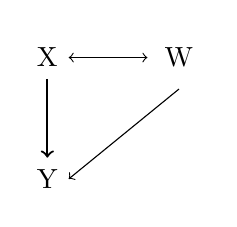
\begin{tikzpicture}[
roundnode/.style={circle, very thick, minimum size=7mm},
squarednode/.style={rectangle, very thick, minimum size=5mm},
]
%Nodes
\node[squarednode] (x)              {X};
\node[roundnode]   (u) [right=of x] {W};
\node[squarednode] (y) [below=of x] {Y};

%Lines
\draw[->, thick] (x.south) -- (y.north);
\draw[<->] (x.east) --  (u.west);
%\draw[<-] (y.east) --  (u.south);
\draw[->] (u.south) -- (y.east);
\end{tikzpicture}
\caption{Dual Path Causal Graph}
\label{fig:mult}
\end{figure}

Longer regressions do not always reach a correct solution.
Figure \ref{fig:mult} illustrates the problem. 
The figure shows a confounded linear model in which two distinct causal pathways for X on Y exist. 
There is a direct causal effect of X on Y and an indirect causal effect of X on Y, which is mediated by W.
Our ultimate goal is to estimate all three parameters. 
So of particular interest is determining whether or not $b = 0$.
However, as shown in the figure, a backdoor relationship affecting Y through W would overestimate b.

In such a causal relationship, 
if all causal-related variables are omitted and 
the model is constructed with only the variable relationships between the target and response variables; then, the model suffers from omitted variable bias.
Conversely, if more predictors are added, and yet each variable is correlated with each other, 
the problem of multicollinearity arises.

Figure \ref{fig:mult} shows that x and w are causally related and therefore correlated. 
In other words, "causality implies correlation." 
This correlation between independent variables makes it difficult for the algorithm to separate the effect of x on y from the effect of w on y.
When multiple causal relationships exist, it is difficult to express them in only one regression equation.

% \subsubsection*{OLS Model}
% <<>>=
% y <- x1$lwage76
% X <- cbind(1,x1$ed76, x1$exp, x1$exp2, x1$black, x1$reg76r,
%            x1$smsa76r, x1$smsa66r, x1$reg662, x1$reg663,
%            x1$reg664, x1$reg665, x1$reg666, x1$reg667,
%            x1$reg668, x1$reg669)
% beta_ols <- solve(t(X)%*%X)%*%t(X)%*%y
% beta_ols
% @

\subsubsection*{Check Assumptions}
As shown in OLS model, there are four assumptions in linear regression model about the data.

(1) \textbf{Linearity of the data}

The relationship between the predictor (x) and the outcome (y) is assumed to be linear.

(2) \textbf{Normality of residuals}

The residual errors are assumed to be normally distributed.

(3) \textbf{homoscedasticity}

The residuals are assumed to have a constant variance (Homogeneity of residuals variance).

(4) \textbf{Independence of residuals error terms}

In these assumptions, we should check whether or not these assumptions hold true. 

Potential problems include:

(1) \emph{Non-linearity} of the outcome - predictor relationships

(2) \emph{Heteroscedasticity}: Non-constant variance of error terms.

(3) \emph{Presence of influential values} in the data that can be:

\underline{Outliers}: extreme values in the outcome (y) variable

\underline{High-leverage points}: extreme values in the predictors (x) variable

All these assumptions and potential problems can be checked by producing some diagnostic plots visualizing the residual errors.

\begin{knitrout}
\definecolor{shadecolor}{rgb}{0.969, 0.969, 0.969}\color{fgcolor}\begin{kframe}
\begin{alltt}
\hlcom{# Check Multilinear Regression Assumptions}
\hlkwd{par}\hlstd{(}\hlkwc{mfrow} \hlstd{=} \hlkwd{c}\hlstd{(}\hlnum{2}\hlstd{,} \hlnum{2}\hlstd{))}
\hlkwd{plot}\hlstd{(lm.both)}
\end{alltt}


{\ttfamily\noindent\bfseries\color{errorcolor}{\#\# Error in h(simpleError(msg, call)): error in evaluating the argument 'x' in selecting a method for function 'plot': object 'lm.both' not found}}\end{kframe}
\end{knitrout}

Overall, there is nothing serious problem to violate the assumptions.

\newpage
\subsection*{IV Model}
% Basic IV model
The instrumental variable estimator (IV estimator) is the most common technique to solve the confounding model in econometrics or epidemiology \citep{klungel2015instrumental}.
IV model is used when controlled experiments are not feasible or when a treatment is not successfully delivered to every unit in a randomized experiment.
Figure \ref{fig:iv} shows that the instrumental variable (Z) has a direct causal effect on X 
but is not determined by the unobserved characteristic. 
There is an arrow from Z to X and an arrow from U to X, but no arrow from U to Z.

Intuitively, IV is used when the explanatory variable of interest is correlated with the error term, and ordinary least squares or ANOVA would yield biased results.
An effective instrument can reveal the causal effect of the explanatory variable on the dependent variable because it induces a change in the explanatory variable but has no independent effect on the dependent variable.


% IV model graph
\begin{figure}[htp]
\centering
\begin{tikzpicture}[
roundnode/.style={circle, very thick, minimum size=7mm},
squarednode/.style={rectangle, very thick, minimum size=5mm},
]
%Nodes
\node[squarednode] (x)              {X};
\node[squarednode] (z) [above=of x] {Z};
\node[roundnode]   (u) [right=of x] {U};
\node[squarednode] (y) [below=of x] {Y};

%Lines
\draw[->] (z.south) -- (x.north);
\draw[->, thick] (x.south) -- (y.north);
\draw[<-] (x.east) --  (u.west);
\draw[<-] (y.east) --  (u.south);
\draw[->] (u.south) -- (y.east);
\end{tikzpicture}
\caption{IV Causal Graph}
\label{fig:iv}
\end{figure}

An IV estimator is derived by a structural equation model \citep{bielby1977structural}, which is in general:
\begin{align*}
y&=f_y(x,e_U)\\
x&=f_x(z,e_U).
\end{align*}

This equations represents that 
the value of variable y is determined by a function, $f_y$, 
the value of variable $x$ and the error variable $e_U$, and 
the value of variable $x$ is determined by 
a function, $f_x$, of the value of an instrumental variable $Z$ and 
the error variable $e_U$ on the right side.

However, most of the case, we assume the linear model in the parameter $\beta$; 
so rearranging the equation above into a matrix algebra:
\begin{align*}
\mathbf{y}&=\mathbf{X}\beta+v\\
\mathbf{X}&=\mathbf{Z}\Delta+\mathbf{E},
\end{align*}
where $\mathbf{y}$ is a one-dimensional vector of the outcome of interest $\mathbf{y}$, $\mathbf{X}$ is a matrix of the observed explanatory variables $\{1, x_i\}$, $\beta$ is a vector of the model parameters, and $v$ is a one-dimensional vector of the error term $v_i$ for the first equation.
In addition, $\mathbf{Z}$ is a matrix of the instrumental variables $\{1, z_i\}$, $\Delta$ is a matrix of the relationship between the explanatory variables and the instrumental variables, and $E$ is a matrix of unobserved characteristics determining the explanatory variables.

We can shuffle the matrix equations, and obtain:
$$\beta = \left(\mathbf{Z}^T\mathbf{X}\right)^{-1}\mathbf{Z}^T\mathbf{y} - 
\left(\mathbf{Z}^T\mathbf{X}\right)^{-1}\mathbf{Z}^T\mathbf{v}.$$

Since we assume that the expected value of error term is zero, we obtain the instrumental variable estimator:
$$\hat\beta_{IV}=\left(\mathbf{Z}^T\mathbf{X}\right)^{-1}\mathbf{Z}^T\mathbf{y}$$
% Properties
\subsubsection*{Properties of IV Estimator}
In order to set an ideal instrumental variable, it must satisfy three properties \citep{angrist2014mastering}:
\begin{enumerate}[itemsep=-5mm]
  \item The variable directly affects the policy variable of interest (Z → X).\\
  \item The variable is independent of the unobserved characteristics that
affect the policy variable and the outcome of interest ($U \not\to Z$).\\
  \item The variable affects the policy variable independently of the unobserved effect ($X = dZ + U$).
\end{enumerate}

Given a variable that satisfies these three properties, 
IV estimator can be used to estimate the desired causality.

% Card's Argument
Now we are back to the discussion of how Card used OLS to estimate returns to schooling. 
Card finds that an extra year of schooling increases income by approximately $7.5\%$. 
The unobserved characteristics of the young men may determine both the amount of education that they get and the income they earn. 
In Figure \ref{fig:ivCard}, the problem is illustrated with a causal arrow running from the unobserved characteristic to both income and education.

According to \cite{christofides1995aspects}, Card argues that young ones who grow up near a 4-year university will have lower costs of attending college and are thus more likely to get another year of education. 
Also, Card argues that growing up close to a 4-year college is unlikely to be determined by unobserved characteristics that also determine the amount of education that the young man gets and the income that the young man earns \citep{card2001estimating}. 
In the graph, 
the assumption is represented as an arrow from distance to college to education and no arrow from unobserved characteristics to distance to college.


% Card's IV model graph
\begin{figure}[htp]
\centering
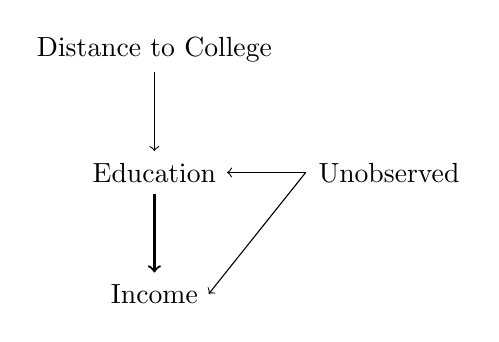
\begin{tikzpicture}[
roundnode/.style={circle, very thick, minimum size=7mm},
squarednode/.style={rectangle, very thick, minimum size=5mm},
]
%Nodes
\node[squarednode] (x)              {Education};
\node[squarednode] (z) [above=of x] {Distance to College};
\node[roundnode]   (u) [right=of x] {Unobserved};
\node[squarednode] (y) [below=of x] {Income};

%Lines
\draw[->] (z.south) -- (x.north);
\draw[->, thick] (x.south) -- (y.north);
\draw[<-] (x.east) --  (u.west);
\draw[<-] (y.east) --  (u.west);
\end{tikzpicture}
\caption{IV Causal Graph for Returning School}
\label{fig:ivCard}
\end{figure}


% Models
Multiple instruments are used by Card, where instruments for experience, as well as the distance to college \citep{christofides1995aspects}. 
Experience is measured as the difference between age and years of education, 
but education is confounded. 
The paper also utilizes age as the instrument for experience and squared age as the instrument for experience-squared.
The instrumental variable procedure derived above is used to estimate the returns to schooling, accounting for all three instruments.

% Empirical analysis
\begin{kframe}
\begin{alltt}
\hlcom{# Data set for income}
\hlstd{y} \hlkwb{<-} \hlstd{x1}\hlopt{$}\hlstd{lwage76}
\end{alltt}


{\ttfamily\noindent\bfseries\color{errorcolor}{\#\# Error in eval(expr, envir, enclos): object 'x1' not found}}\begin{alltt}
\hlcom{# Data set for observed matrix}
\hlstd{X} \hlkwb{<-} \hlkwd{cbind}\hlstd{(}\hlnum{1}\hlstd{,x1}\hlopt{$}\hlstd{ed76, x1}\hlopt{$}\hlstd{exp, x1}\hlopt{$}\hlstd{exp2, x1}\hlopt{$}\hlstd{black, x1}\hlopt{$}\hlstd{reg76r,}
           \hlstd{x1}\hlopt{$}\hlstd{smsa76r, x1}\hlopt{$}\hlstd{smsa66r, x1}\hlopt{$}\hlstd{reg662, x1}\hlopt{$}\hlstd{reg663,}
           \hlstd{x1}\hlopt{$}\hlstd{reg664, x1}\hlopt{$}\hlstd{reg665, x1}\hlopt{$}\hlstd{reg666, x1}\hlopt{$}\hlstd{reg667,}
           \hlstd{x1}\hlopt{$}\hlstd{reg668, x1}\hlopt{$}\hlstd{reg669)}
\end{alltt}


{\ttfamily\noindent\bfseries\color{errorcolor}{\#\# Error in cbind(1, x1\$ed76, x1\$exp, x1\$exp2, x1\$black, x1\$reg76r, x1\$smsa76r, : object 'x1' not found}}\begin{alltt}
\hlcom{# Data set for instrumental variables}
\hlstd{Z1} \hlkwb{<-} \hlkwd{cbind}\hlstd{(}\hlnum{1}\hlstd{,x1}\hlopt{$}\hlstd{nearc4, x1}\hlopt{$}\hlstd{age76, x1}\hlopt{$}\hlstd{age2, x1}\hlopt{$}\hlstd{black,}
            \hlstd{x1}\hlopt{$}\hlstd{reg76r,x1}\hlopt{$}\hlstd{smsa76r, x1}\hlopt{$}\hlstd{smsa66r, x1}\hlopt{$}\hlstd{reg662,}
            \hlstd{x1}\hlopt{$}\hlstd{reg663,x1}\hlopt{$}\hlstd{reg664, x1}\hlopt{$}\hlstd{reg665, x1}\hlopt{$}\hlstd{reg666,}
            \hlstd{x1}\hlopt{$}\hlstd{reg667, x1}\hlopt{$}\hlstd{reg668, x1}\hlopt{$}\hlstd{reg669)}
\end{alltt}


{\ttfamily\noindent\bfseries\color{errorcolor}{\#\# Error in cbind(1, x1\$nearc4, x1\$age76, x1\$age2, x1\$black, x1\$reg76r, x1\$smsa76r, : object 'x1' not found}}\begin{alltt}
\hlcom{# Estimate the instrumental variable estimator}
\hlstd{invZTX} \hlkwb{<-} \hlkwd{solve}\hlstd{(}\hlkwd{t}\hlstd{(Z1)}\hlopt\hlstd{X)}
\end{alltt}


{\ttfamily\noindent\bfseries\color{errorcolor}{\#\# Error in t(Z1): object 'Z1' not found}}\begin{alltt}
\hlstd{ZTy}    \hlkwb{<-} \hlkwd{t}\hlstd{(Z1)}\hlopt\hlstd{y}
\end{alltt}


{\ttfamily\noindent\bfseries\color{errorcolor}{\#\# Error in t(Z1): object 'Z1' not found}}\begin{alltt}
\hlstd{beta_iv}\hlkwb{<-} \hlstd{invZTX}\hlopt\hlstd{ZTy}
\end{alltt}


{\ttfamily\noindent\bfseries\color{errorcolor}{\#\# Error in eval(expr, envir, enclos): object 'invZTX' not found}}\begin{alltt}
\hlcom{## Calculate t statistics for significance test}
\hlcom{# calculate sigma squared hat}
\hlstd{N}\hlkwb{=}\hlkwd{length}\hlstd{(y)}
\end{alltt}


{\ttfamily\noindent\bfseries\color{errorcolor}{\#\# Error in eval(expr, envir, enclos): object 'y' not found}}\begin{alltt}
\hlstd{k}\hlkwb{=}\hlkwd{ncol}\hlstd{(X)}\hlopt{-}\hlnum{1}
\end{alltt}


{\ttfamily\noindent\bfseries\color{errorcolor}{\#\# Error in ncol(X): object 'X' not found}}\begin{alltt}
\hlstd{sigma2} \hlkwb{<-} \hlkwd{t}\hlstd{(y} \hlopt{-} \hlstd{X} \hlopt \hlstd{beta_iv)} \hlopt \hlstd{(y} \hlopt{-} \hlstd{X} \hlopt \hlstd{beta_iv)} \hlopt{/} \hlstd{(N}\hlopt{-}\hlstd{k}\hlopt{-}\hlnum{1}\hlstd{)}
\end{alltt}


{\ttfamily\noindent\bfseries\color{errorcolor}{\#\# Error in t(y - X \%*\% beta\_iv): object 'y' not found}}\begin{alltt}
\hlcom{# allocate the lists of standard error and t stat for alpha}
\hlstd{se.b} \hlkwb{<-} \hlstd{t.b}  \hlkwb{<-} \hlkwd{c}\hlstd{(}\hlkwd{rep}\hlstd{(}\hlnum{0}\hlstd{,k}\hlopt{+}\hlnum{1}\hlstd{))}
\end{alltt}


{\ttfamily\noindent\bfseries\color{errorcolor}{\#\# Error in eval(expr, envir, enclos): object 'k' not found}}\begin{alltt}
\hlcom{# calculate standard error for estimates}
\hlkwa{for} \hlstd{(i} \hlkwa{in} \hlnum{1}\hlopt{:}\hlstd{(k}\hlopt{+}\hlnum{1}\hlstd{))\{}
  \hlstd{se.b[i]} \hlkwb{<-} \hlkwd{sqrt}\hlstd{(sigma2} \hlopt{*} \hlstd{invZTX[i,i])}
\hlstd{\}}
\end{alltt}


{\ttfamily\noindent\bfseries\color{errorcolor}{\#\# Error in eval(expr, envir, enclos): object 'k' not found}}\begin{alltt}
\hlcom{# calculate t statistics for each estimates}
\hlkwa{for} \hlstd{(i} \hlkwa{in} \hlnum{1}\hlopt{:}\hlstd{(k}\hlopt{+}\hlnum{1}\hlstd{))\{}
  \hlstd{t.b[i]} \hlkwb{<-} \hlstd{beta_iv[i]}\hlopt{/}\hlstd{se.b[i]}
\hlstd{\}}
\end{alltt}


{\ttfamily\noindent\bfseries\color{errorcolor}{\#\# Error in eval(expr, envir, enclos): object 'k' not found}}\begin{alltt}
\hlcom{# critical value at significant level 0.05}
\hlstd{cv025} \hlkwb{<-} \hlkwd{qt}\hlstd{(}\hlnum{0.975}\hlstd{, N}\hlopt{-}\hlstd{k}\hlopt{-}\hlnum{1}\hlstd{,} \hlkwc{lower.tail}\hlstd{=}\hlnum{TRUE}\hlstd{)}
\end{alltt}


{\ttfamily\noindent\bfseries\color{errorcolor}{\#\# Error in qt(0.975, N - k - 1, lower.tail = TRUE): object 'N' not found}}\begin{alltt}
\hlcom{# show beta_iv and cv}
\hlstd{beta_iv_cv}\hlkwb{<-}\hlkwd{data.frame}\hlstd{(}\hlkwc{coef}\hlstd{=}\hlkwd{c}\hlstd{(beta_iv),}\hlkwc{se}\hlstd{=}\hlkwd{c}\hlstd{(se.b),}
                       \hlkwc{cv05}\hlstd{=}\hlkwd{c}\hlstd{(beta_iv}\hlopt{-}\hlstd{cv025}\hlopt{*}\hlstd{se.b),}\hlkwc{cv95}\hlstd{=}\hlkwd{c}\hlstd{(beta_iv}\hlopt{+}\hlstd{cv025}\hlopt{*}\hlstd{se.b),}
           \hlkwc{row.names} \hlstd{=} \hlkwd{c}\hlstd{(}\hlstr{"intercept"}\hlstd{,}\hlstr{"ed76"}\hlstd{,}\hlstr{"exp"}\hlstd{,}\hlstr{"exp2"}\hlstd{,}\hlstr{"black"}\hlstd{,}\hlstr{"reg76r"}\hlstd{,}
                         \hlstr{"smsa76r"}\hlstd{,}\hlstr{"smsa66r"}\hlstd{,}\hlstr{"reg662"}\hlstd{,}\hlstr{"reg663"}\hlstd{,}\hlstr{"reg664"}\hlstd{,}
                         \hlstr{"reg665"}\hlstd{,}\hlstr{"reg666"}\hlstd{,}\hlstr{"reg667"}\hlstd{,}\hlstr{"reg668"}\hlstd{,}\hlstr{"reg669"}\hlstd{))}
\end{alltt}


{\ttfamily\noindent\bfseries\color{errorcolor}{\#\# Error in data.frame(coef = c(beta\_iv), se = c(se.b), cv05 = c(beta\_iv - : object 'beta\_iv' not found}}\begin{alltt}
\hlkwd{print}\hlstd{(}\hlkwd{xtable}\hlstd{(beta_iv_cv))}
\end{alltt}


{\ttfamily\noindent\bfseries\color{errorcolor}{\#\# Error in xtable(beta\_iv\_cv): object 'beta\_iv\_cv' not found}}\end{kframe}

The instrumental variable estimates for returns to schooling are substantially higher than the OLS estimates. This is contrary to my expectation.
In general, I expected the OLS estimates of the causal effect of schooling on income to be biased upward.
The concern is that the OLS might be picking up on the fact that the family environment determines both college attendance and access to higher-earning jobs. 
This result suggests that the OLS estimates are biased downward. 
The reason for the upward bias of the instrumental variable estimates will be clarified in future studies, 
since this is a comparison of three models: OLS, the instrumental variable estimation, and LiNGAM.

Note that the equations of interest for the instrumental variable method are structural, not regression.
So, the validation of the assumptions is different from the usual regression model.

\newpage
\subsection*{LiNGAM}
% LiNGAM 
The instrumental variables (IV) method is one of the causal discoveries in statistics.
It is used to estimate causal relationships, utilizing a structural equation modelling (SEM), 
when controlled experiments are not feasible or when a treatment is not successfully delivered to every unit in a randomized experiment.
\cite{shimizu2006linear} introduced a non-Gaussian version of the linear acyclic SEM 
with no latent confounders, known as a linear non-Gaussian acyclic model, abbreviated as LiNGAM:
$$x_i=\sum_{k(j)<k(i)}b_{ij}x_j+e_i$$
where $e_i$ are exogenously latent variables, and $b_{ij}$ are the connection strengths from $x_j$ to $x_i$. 
With the causal ordering of the variables $x_i$, denoted by $k(i)$, 
the causal relations of the variables $x_i$ can be graphically represented by using a directed acyclic graph in Figure \ref{fig:l}. 
The exogenous variables $e_i$ follow non-Gaussian distributions but one of $e_i$ at most Gaussian, 
with zero mean and non-zero variance and are mutually independent. 
The independence assumption between $e_i$ implies that there are no latent confounding variables. 
In matrix form, the LiNGAM model is written as:

$$\mathbf{x} = \mathbf{B}\mathbf{x}+\mathbf{e}$$

where the matrix $\mathbf{B}$ collects the connection strengths $b_{ij}$ , 
and the vectors $\mathbf{x}$ and $\mathbf{e}$ collect the observed variables $x_i$ and the exogenous variables $e_i$, respectively.

% LiNGAM Graph
\begin{figure}[htp]
\centering
\begin{tikzpicture}[
roundnode/.style={circle, very thick, minimum size=7mm},
squarednode/.style={rectangle, very thick, minimum size=5mm},
]
%Nodes
\node[squarednode] (x)              {X};
\node[squarednode] (z) [below left  = 2.3cm and 1.5cm of x] {Y};
\node[squarednode] (y) [below right = 2.3cm and 1.5cm of x] {Z};
\node[roundnode]   (u) [above=of x] {U};
\node[roundnode]   (v) [right=of y] {V};
\node[roundnode]   (w) [left=of z]  {W};

%Lines
\draw[<->, thick] (x.east) -- (y.north);
\draw[<->, thick] (x.west) -- (z.north);
\draw[<->, thick] (y.west) -- (z.east);

\draw[->] (u.south)--(x.north);
\draw[->] (v.west) --(y.east);
\draw[->] (w.east) --(z.west);
\end{tikzpicture}
\caption{Directed Acyclic Graph (Causal Pathway)}
\label{fig:l}
\end{figure}

According to \cite{shimizu2014lingam}, the fundamental concept of LiNGAM and its estimation is closely related to the independent component analysis (ICA).
ICA is a non-Gaussian variant of factor analysis, and the ICA model for the observed variables $x_i$ can be defined as follows:
$$x_i=\sum_{j=1}^da_{ij}s_j$$

We do not go beyond the detail of ICA and how to solve using ICA and work the algorithm to its estimation. 

\subsubsection*{Assumptions to LiNGAM}
LiNGAM has the basic four assumptions \citep{shimizu2006linear}:

\begin{enumerate}[itemsep=-5mm]
  \item Linearity: simplified model in this case but can be extended\\
  \item Acyclicity: causal structure (Parent-child relationship of the data variables)\\
  \item Non-Gaussian: semi-parametric or at most one is Gaussian error distribution\\
  \item Markov Property: all nodes are independent of their non-descendants when conditioned on their parents\\
\end{enumerate}

The major difference between LiNGAM and the estimation method of the instrumental variables is:
LiNGAM is computationally capable of performing a causal search without human intervention, while IV is in that the researcher constructs the IV, and causal inference is made statistically from its structural equations.

% Application to Card's case
So we would like to apply LiNGAM estimation to the Card’s data of returns of schooling.
The data used is the same data used in Multiple regression and IV estimation.
The LiNGAM estimation method uses the R package of "pcalg: Methods for Graphical Models and Causal Inference" \footnote{https://cran.r-project.org/web/packages/pcalg/pcalg.pdf} to estimate the connection strength matrix $\mathbf{B}$. 

The R code and the resulting matrix $\mathbf{B}$ is shown below.

\begin{knitrout}
\definecolor{shadecolor}{rgb}{0.969, 0.969, 0.969}\color{fgcolor}\begin{kframe}
\begin{alltt}
\hlcom{# Data setup}
\hlstd{X} \hlkwb{<-} \hlkwd{cbind}\hlstd{(x1}\hlopt{$}\hlstd{lwage76, x1}\hlopt{$}\hlstd{ed76, x1}\hlopt{$}\hlstd{exp, x1}\hlopt{$}\hlstd{exp2, x1}\hlopt{$}\hlstd{black, x1}\hlopt{$}\hlstd{reg76r,}
           \hlstd{x1}\hlopt{$}\hlstd{smsa76r, x1}\hlopt{$}\hlstd{smsa66r, x1}\hlopt{$}\hlstd{reg662, x1}\hlopt{$}\hlstd{reg663,}
           \hlstd{x1}\hlopt{$}\hlstd{reg664, x1}\hlopt{$}\hlstd{reg665, x1}\hlopt{$}\hlstd{reg666, x1}\hlopt{$}\hlstd{reg667,}
           \hlstd{x1}\hlopt{$}\hlstd{reg668, x1}\hlopt{$}\hlstd{reg669)}
\end{alltt}


{\ttfamily\noindent\bfseries\color{errorcolor}{\#\# Error in cbind(x1\$lwage76, x1\$ed76, x1\$exp, x1\$exp2, x1\$black, x1\$reg76r, : object 'x1' not found}}\begin{alltt}
\hlcom{# LiNGAM function to estimate causal discoveries}
\hlstd{lingam.res} \hlkwb{<-} \hlkwd{lingam}\hlstd{(X,} \hlkwc{verbose} \hlstd{=} \hlnum{2}\hlstd{)}
\end{alltt}


{\ttfamily\noindent\bfseries\color{errorcolor}{\#\# Error in ncol(X): object 'X' not found}}\end{kframe}
\end{knitrout}
\begin{kframe}
\begin{alltt}
\hlcom{# as(lingam.res, "amat")}
\hlcom{# display the connection strenght matrix}
\hlkwd{print}\hlstd{(}\hlkwd{xtable}\hlstd{(lingam.res}\hlopt{$}\hlstd{Bpruned,} \hlkwc{type} \hlstd{=} \hlstr{"latex"}\hlstd{))}
\end{alltt}


{\ttfamily\noindent\bfseries\color{errorcolor}{\#\# Error in xtable(lingam.res\$Bpruned, type = "{}latex"{}): object 'lingam.res' not found}}\end{kframe}

\begin{figure}[htp]
\centering
\resizebox{0.5\textwidth}{!}{%
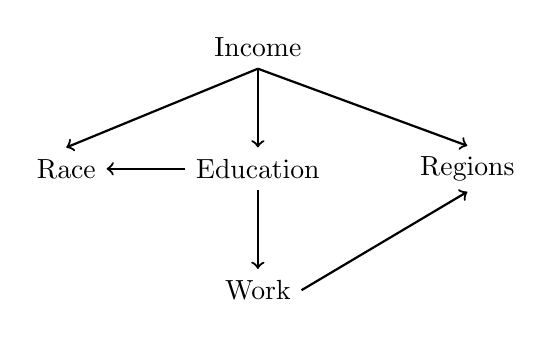
\begin{tikzpicture}[roundnode/.style={circle, very thick, minimum size=7mm},
                    squarednode/.style={rectangle, very thick, minimum size=5mm}
                   ]
%Nodes
\node[squarednode] (1)               {Income};
\node[squarednode] (2)  [below=of 1] {Education};
\node[squarednode] (34) [below=of 2] {Work};
\node[squarednode] (5)  [left =of 2] {Race};
\node[squarednode] (678)[right=of 2] {Regions};
% %Lines
\draw[->, thick] (1.south) -- (2.north);
\draw[->, thick] (1.south) -- (5.north);
\draw[->, thick] (1.south) -- (678.north);

\draw[->, thick] (2.west) -- (5.east);

\draw[->, thick] (2.south)--(34.north);
\draw[->, thick] (34.east) --(678.south);
\end{tikzpicture}
}
\caption{Directed Acyclic Graph of Returning to School}
\label{fig:resG}
\end{figure}

A causal graph from the estimated connection strength matrix yielded results that contradicted my expectations.
In this graph, to simplify the graph, I grouped the following variables together and eliminated the non-connected variables.
Two of $\{exp\}$ and $\{exp2\}$ is grouped to $\{work\}$, three of $\{reg76r\}$, $\{smsa76r\}$, and $\{smsa66r\}$ is a set to $\{regions\}$.
The causality graph suggests that 
"income" affects "education," "race," and "years of employment";
"education" affects "race" and "years of employment";
and "years of employment" affects "area of residence." 
The results are the opposite of the commonly accepted causal relationship.

\newpage

\section{Discussion and Conclusion}

This paper represents the comparison of the estimations of higher education on individual income levels, 
using microeconomic survey data on men aged between 14 and 24 in 1966, with four statistical models:
(1) Simple Linear Regression, (2) Multiple Linear Regression, (3) the Instrumental Variable Estimation, and (4) Linear Non-Gaussian Acyclic Model.

Under the standard T testing approach, we cannot reject that the estimated parameter, the effect of schooling on income, every linear regression model is zero.
Furthermore, there are no severe issues with each linear regression's assumptions.

\begin{kframe}


{\ttfamily\noindent\bfseries\color{errorcolor}{\#\# Error in data.frame(simple = c(lm1\$coefficients[1], lm1\$coefficients[2], : object 'lm1' not found}}

{\ttfamily\noindent\bfseries\color{errorcolor}{\#\# Error in xtable(comp, type = "{}latex"{}): object 'comp' not found}}\end{kframe}

% beta estimation
In all models, it is an implication that education in school has a relationship to income. 
In other words, on average, an association between schooling and individual income typically exists. 
The IV model reveals a possibility that education may have an impact on income using college proximity as an instrumental variable.
However, the effect showed different results in each model. 
The single regression analysis estimated a smaller relationship between college education and income than 
the multiple regression analysis. 
Perhaps the simple regression suffers from an omitted variable bias, 
the relationship between education and income was more extensive when variables other than education, such as years of work, were added to the regression model.

An introduction of the instrumental variable method, however, called the relationship into question. 
The result of the instrumental variable estimate the effect of schooling to returns substantially higher than the OLS estimates.
Because what the IV results show is that the influence relationship between each other by OLS is biased downward. 
In many studies, the introduction of the instrumental variable method has strengthened the causal relationship,
but our IV model has weakened it for education and income. 
Whether this is due to a problem in the setting of the control variables or a problem in the structural equations awaits future detailed study.

A more interesting result is that when the recently developed LiNGAM is applied to the Card's data, 
it indicates the opposite of the common-sense causal relationship.
That is, income may have an effect on education.
This experimental result was obtained in this study because the data were directly applied to the LiNGAM model without considering time constraints among variables. 
In future studies, it is expected that introducing a temporal constraint condition will result in a more accurate statistical causal search.
Despite being young history, causal discovery is a promising field that may help bridge the gap between machine and human knowledge.

%% Refernce List
\begin{filecontents}{s673projref.bib} 
@article{shimizu2006linear,
  title={A linear non-Gaussian acyclic model for causal discovery.},
  author={Shimizu, Shohei},
  journal={Journal of Machine Learning Research},
  volume={7},
  number={10},
  year={2006}
}
@article{shimizu2014lingam,
  title={LiNGAM: Non-Gaussian methods for estimating causal structures},
  author={Shimizu, Shohei},
  journal={Behaviormetrika},
  volume={41},
  number={1},
  pages={65--98},
  year={2014},
  publisher={Springer}
}
@article{klungel2015instrumental,
  title={Instrumental variable analysis in epidemiologic studies: an overview of the estimation methods},
  author={Klungel, OH and Uddin, M Jamal and de Boer, A and Belitser, SV and Groenwold, RH and Roes, KC and others},
  journal={Pharm Anal Acta},
  volume={6},
  number={353},
  pages={2},
  year={2015}
}
@article{card2001estimating,
  title={Estimating the return to schooling: Progress on some persistent econometric problems},
  author={Card, David},
  journal={Econometrica},
  volume={69},
  number={5},
  pages={1127--1160},
  year={2001},
  publisher={Wiley Online Library}
}
@book{christofides1995aspects,
  title={Aspects of labour market behaviour: Essays in honour of John Vanderkamp},
  author={Christofides, Loizos Nicolaou and Grant, E Kenneth and Vanderkamp, John and Swidinsky, Robert},
  year={1995},
  publisher={University of Toronto Press}
}
@book{angrist2014mastering,
  title={Mastering'metrics: The path from cause to effect},
  author={Angrist, Joshua D and Pischke, J{\"o}rn-Steffen},
  year={2014},
  publisher={Princeton university press}
}
@article{bielby1977structural,
  title={Structural equation models},
  author={Bielby, William Thomas and Hauser, Robert Mason},
  journal={Annual review of sociology},
  volume={3},
  number={1},
  pages={137--161},
  year={1977},
  publisher={Annual Reviews 4139 El Camino Way, PO Box 10139, Palo Alto, CA 94303-0139, USA}
}
@article{chalmers1981method,
  title={A method for assessing the quality of a randomized control trial},
  author={Chalmers, Thomas C and Smith Jr, Harry and Blackburn, Bradley and Silverman, Bernard and Schroeder, Biruta and Reitman, Dinah and Ambroz, Alexander},
  journal={Controlled clinical trials},
  volume={2},
  number={1},
  pages={31--49},
  year={1981},
  publisher={Elsevier}
}
@article{banerjee2016influence,
  title={The influence of randomized controlled trials on development economics research and on development policy},
  author={Banerjee, Abhijit Vinayak and Duflo, Esther and Kremer, Michael},
  journal={The state of Economics, the state of the world},
  pages={482--488},
  year={2016},
  publisher={PublicAffairs}
}
@techreport{mann1949analysis,
  title={Analysis and design of experiments: Analysis of variance and analysis of variance designs},
  author={Mann, Henry Berthold},
  year={1949}
}
@article{stock2003retrospectives,
  title={Retrospectives: Who invented instrumental variable regression?},
  author={Stock, James H and Trebbi, Francesco},
  journal={Journal of Economic Perspectives},
  volume={17},
  number={3},
  pages={177--194},
  year={2003}
}
@incollection{dinardo2010natural,
  title={Natural experiments and quasi-natural experiments},
  author={DiNardo, John},
  booktitle={Microeconometrics},
  pages={139--153},
  year={2010},
  publisher={Springer}
}
@article{lousdal2018introduction,
  title={An introduction to instrumental variable assumptions, validation and estimation},
  author={Lousdal, Mette Lise},
  journal={Emerging themes in epidemiology},
  volume={15},
  number={1},
  pages={1--7},
  year={2018},
  publisher={BioMed Central}
}
@misc{hernan2010causal,
  title={Causal inference},
  author={Hern{\'a}n, Miguel A and Robins, James M},
  year={2010},
  publisher={CRC Boca Raton, FL;}
}
@misc{card1993using,
  title={Using geographic variation in college proximity to estimate the return to schooling},
  author={Card, David},
  year={1993},
  publisher={National Bureau of Economic Research Cambridge, Mass., USA}
}
\end{filecontents}

\newpage
\singlespacing
\bibliography{s673projref}

\end{document}
